% Figure 1: the five-phase APIP lifecycle. Build: pdflatex fig1_apip_lifecycle.tex
\documentclass[tikz,border=2pt]{standalone}
\usetikzlibrary{arrows.meta,positioning,calc}
\begin{document}
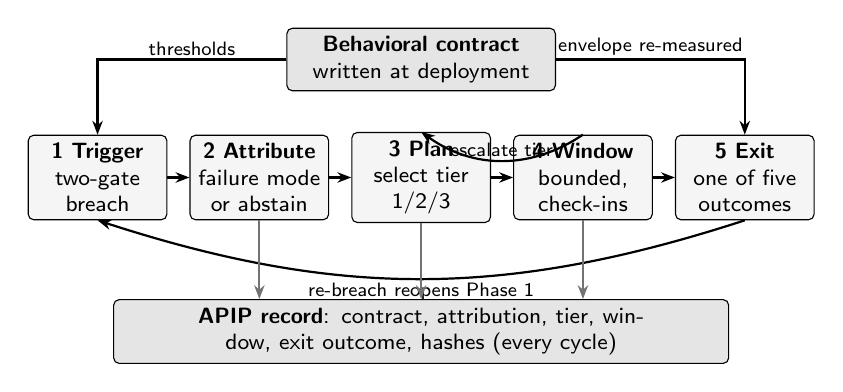
\begin{tikzpicture}[font=\sffamily\footnotesize,
  phase/.style={draw,rounded corners=2pt,minimum height=0.95cm,text width=1.55cm,align=center,inner sep=3pt,fill=black!4},
  ctr/.style={draw,rounded corners=2pt,minimum height=0.6cm,text width=3.2cm,align=center,inner sep=3pt,fill=black!10},
  rec/.style={draw,rounded corners=2pt,minimum height=0.6cm,text width=7.6cm,align=center,inner sep=3pt,fill=black!10},
  arr/.style={-{Stealth[length=5pt]},thick},
  lbl/.style={font=\sffamily\scriptsize,inner sep=1pt}]
  \node[phase] (p1) {\textbf{1 Trigger}\\two-gate breach};
  \node[phase,right=0.28cm of p1] (p2) {\textbf{2 Attribute}\\failure mode or abstain};
  \node[phase,right=0.28cm of p2] (p3) {\textbf{3 Plan}\\select tier 1/2/3};
  \node[phase,right=0.28cm of p3] (p4) {\textbf{4 Window}\\bounded, check-ins};
  \node[phase,right=0.28cm of p4] (p5) {\textbf{5 Exit}\\one of five outcomes};
  \draw[arr] (p1) -- (p2); \draw[arr] (p2) -- (p3); \draw[arr] (p3) -- (p4); \draw[arr] (p4) -- (p5);
  \node[ctr,above=0.55cm of $(p1.north)!0.5!(p5.north)$] (c) {\textbf{Behavioral contract}\\written at deployment};
  \draw[arr] (c.west) -| node[lbl,pos=0.25,above] {thresholds} (p1.north);
  \draw[arr] (c.east) -| node[lbl,pos=0.25,above] {envelope re-measured} (p5.north);
  \draw[arr] (p4.north) to[bend left=35] node[lbl,above] {escalate tier} (p3.north);
  \draw[arr] (p5.south) to[bend left=18] node[lbl,below] {re-breach reopens Phase 1} (p1.south);
  \node[rec,below=1.0cm of $(p1.south)!0.5!(p5.south)$] (r) {\textbf{APIP record}: contract, attribution, tier, window, exit outcome, hashes (every cycle)};
  \foreach \p in {p2,p3,p4} \draw[arr,black!55] (\p.south) -- ($(\p.south |- r.north)$);
\end{tikzpicture}
\end{document}
